\section{合约的套利定价}
\begin{enumerate}[label=\arabic{section}.\arabic*]
    \item \sol
    \begin{enumerate}[label=\alph*)]
        \item $\displaystyle \frac{110-100}{\e^{0.06\times2}}-10=-1.1308$.
        \item $\displaystyle \frac{0}{\e^{0.06\times2}}-10=-10$.
    \end{enumerate}
    \item \sol
    \begin{enumerate}[label=\alph*)]
        \item $\displaystyle \frac{0}{\e^{0.06\times1/2}}-5=-5$.
        \item $\displaystyle \frac{100-98}{\e^{0.06\times1/2}}-5=-3.059$.
    \end{enumerate}
    \item \sol\\
    利用一价律,有\[S=K\e^{-r}-C \Rightarrow C=S-K\e^{-r}.\]
    \item \pro\\
    若$C>S$,则通过同时卖出看涨期权和购买证券来实现套利.
    \item \sol\\
    由命题5.2.2,有$S+P-C=K\e^{-rt}$,而$P \geq 0$,所以$K\e^{-rt} \geq S-C$.
    \item \sol\\
    由上一题,$C \geq S-K\e^{-rt}=30-28\e^{-0.05/3}=2.4628$.
    \item \sol\\
    由练习5.4,有$C \leq S$,则
    \begin{enumerate}[label=\alph*)]
        \item $P-S=K\e^{-rt}+C-2S$,正负皆有可能,该式不一定成立.
        \item $P-K\e^{-rt}=C-S \leq 0 \Rightarrow P \leq K\e^{-rt} \leq K$,该式一定成立.
    \end{enumerate}
    \item \pro \[P-K\e^{-rt}+S=C \geq 0 \Rightarrow P \geq K\e^{-rt}-S.\]
    \item \pro\\
    在时刻0,卖出一股股票$S$,卖出一个看跌期权$P$,买入一个看涨期权$C$,收入$S+P-C$;\\
    在时刻$t$,若$S(t) \leq K$,卖出的看跌期权无用,看涨期权被执行,以执行价$K$买入股票;若$S(t) > K$,买入的看涨期权无用,看跌期权被执行,以执行价$K$买入股票.\\
    由于$S+P-C>K\e^{-rt}$,所以$(S+P-C)\e^{rt}-K>0$,即总可以获得正的收益.
    \item \pro
    \begin{itemize}
        \item 在时刻0,买入一股股票$S$,买入一个看跌期权$P$,卖出一个看涨期权$C$,支出$S+P-C$;在时刻$t$,总是收入$K$.
        \item 向银行存入$K\e^{-rt}$,支出$K\e^{-rt}$,收入$K$.
    \end{itemize}
    所以$S+P-C=K\e^{-rt}$.
    \item \sol\\
    设$P$为看跌期权的价格,则
    \begin{enumerate}[label=\alph*)]
        \item 在时刻0,买入看跌期权$P$、证券$s$;在时刻$t$,由于$K>s_1>s_2$,所以卖出看跌期权$K$,所以回报是$K-(P-S)\e^{rt}$.
        \item $K-(P-S)\e^{rt} 0 \Rightarrow P = K\e^{-rt} - s$.
    \end{enumerate}
    \item \sol
    \begin{itemize}
        \item 在时刻0,买入看涨和看跌期权$P$,支出$C_1+C_2$;在时刻1,收入1.
        \item 向银行存入$\e^{-rt}$,支出$\e^{-rt}$,收入1.
    \end{itemize}
    所以$C_1+C_2=\e^{-rt}$.
    \item \sol\\
    因为$25=S+P-C > K\e^{-rt}=20\e^{-0.1/4}$,所以套利策略为在时刻0,卖出证券$S$,卖出看跌期权$P$,买入看涨期权$C$;在时刻$t$,收入$K$. 回报为$(S+P-C)\e^{rt}-K=5.6329$.
    \item \sol\\
    若这些期权均为欧式期权,令其价格分别为$C,P$,则有\[C_a = C, P_a \geq P,\]
    所以\[S+P-C=K\e^{-rt} \Rightarrow S+P_a-C_a \geq K\e^{-rt}.\]
    \item \pro\\
    若$K_1-K_2 < P_1-P_2$,即$K_2-K_1+P_1-P_2>0$,不妨假设$P_1 > P_2$,在时刻0,卖出$(K_1,P_1)$,买入$(K_2,P_2)$,收入$P_1-P_2$;在时刻$t$,若两者均执行,则支出$K_2-K_1$,则$K_2-K_1+P_1-P_2>0$,存在套利机会,产生矛盾,于是$K_1-K_2 \geq P_1-P_2$.
    \item \sol\\
    设某一美式看跌期权$t$时刻的价格为$P_1$,另一个美式看跌期权$s(s<t)$时刻的价格为$P_2$,即证$P_1 \geq P_2$.\\
    若$P_1 < P_2$,买入$(P_1,t)$,卖出$(P_2,s)$,若两者均执行,则此时收入支出相互抵消,获得初始收益$P_2-P_1$,于是存在套利机会,产生矛盾,所以$P_1 \geq P_2$.
    \item \sol
    \begin{enumerate}[label=\alph*)]
        \item 正确,因为$C=S+P-K\e^{-rt}$关于$t$非减,同时该结论对美式看涨期权也成立.
        \item 错误,因为$F=S\e^{(r_u-r_g)t}$,若要关于$t$非减,需要$r_u \geq r_g$,而题中未说明大小关系.
        \item 错误,因为$P=K\e^{-rt}+C-S$关于$t$非增.
    \end{enumerate}
    \item \sol\\
    设欧式看涨期权的价格为$C$,欧式看跌期权的价格为$P$,则$K=S+P-C$
    \begin{enumerate}[label=\alph*)]
        \item 因为$S+P-C - K\e^{-rt}=(S+P-C)(1-\e^{-rt})>0$,回报为$(S+P-C)\e^{rt}-K=(S+P-C)\e^{rt}-(S+P-C)=(S+P-C)(\e^{rt}-1)>0$,所以这个投资策略恒合理.
        \item 函数是$f(C)=(S+P-C)(\e^{r/4}-1)$,图如下:
        \begin{figure}[H]
            \centering
            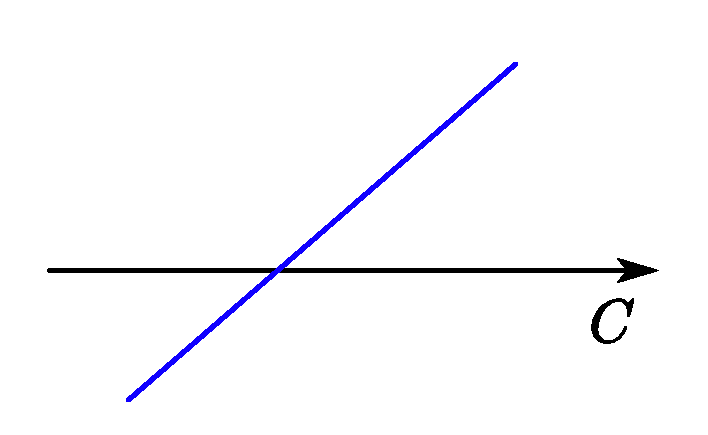
\includegraphics[scale=0.4]{5.18.pdf}
        \end{figure}
    \end{enumerate}
    \item \sol\\ $s-d$.
    \item \sol
    \begin{enumerate}[label=\alph*)]
        \item $(S(t)-K)^++(K-S(t))^+=|S(t)-K|$.
        \item $(S(t)-K_1)^+-(K_2-S(t))^+$.
        \item $2(S(t)-K)^+-S(t)$.
        \item $S(t)-(S(t)-K)^+$.
    \end{enumerate}
    \item \pro\\
    有$C(K)=S+P-K\e^{-rt}$,有$C'(K)=-\e^{-rt}<0$,所以一个欧式看涨期权的价格关于其敲定价是非增的.
    \item \sol
    \begin{enumerate}[label=\alph*)]
        \item $100-105=-5<0$,这个投资的初始成本是负的.
        \item 回报为$f[S(t)]=(S(t)-100)^+-(S(t)-105)^+$,图如下:
        \begin{figure}[H]
            \centering
            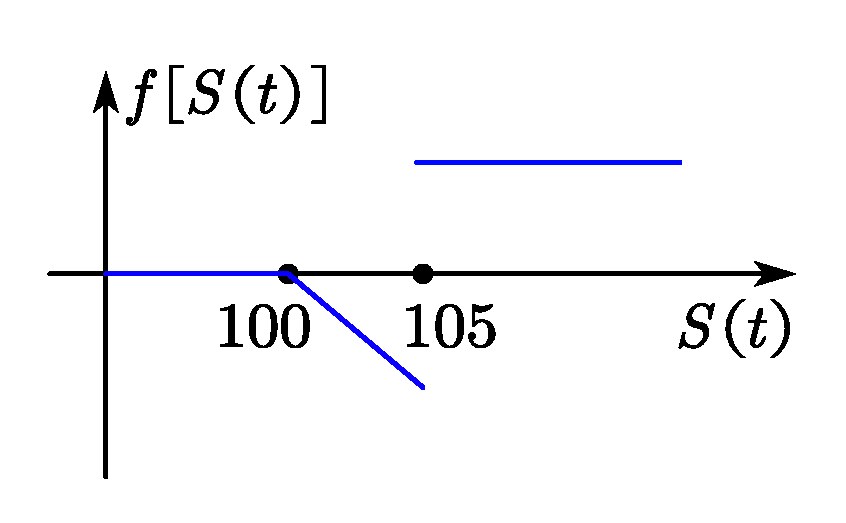
\includegraphics[scale=0.3]{5.22.pdf}
        \end{figure}
    \end{enumerate}
    \item \sol\\
    在时刻0,买入敲定价为110的看涨期权,卖出敲定价为100的看涨期权,收入$20-C$;在时刻$t$,两个看涨期权都执行时,最多支出10,所以$20-C \leq 10\e^{-rt}$,即$C \geq 20-10\e^{-rt}$.
    \item \pro\\ 因为$S+P-C=K\e^{-rt}$,所以$P(K,t)=K\e^{-rt}+C-S$,显然$P(K,t)$对于固定的$t$,关于$K$是凸函数(也是凹函数).
    \item \sol\\ 可以,考虑两个投资
    \begin{itemize}
        \item 购买1份$(K,t)$美式看跌期权;
        \item 购买$\lambda$份$(K_1,t)$美式看跌期权和$(1-\lambda)$份$(K_2,,t)$美式看跌期权.
    \end{itemize}
    其中$K=\lambda K_1+(1-\lambda)K_2$. 当证券价格为$s$时,回报为$(K^*-s)^+$,$K^*$为看跌期权的执行价. 根据回报的凸性,即可得价格的凸性.
    \item \pro\\
    若$t_1$时刻期权价格是$s$,在此时卖出证券,收入$s-K_1$;在$t_2$时刻买回证券,等价于$t_1$时刻收入$s-K_2\e^{-r(t_2-t_1)}$. 因为$K_1>K_2\e^{-r(t_2-t_1)}$,所以$t_1$时刻不会执行该期权.
    \item \pro\\
    由于$-\max\{a,b\}=\min\{-a,-b\}$,则
    \[S(t)-\max\{K,S(t)-A\}=S(t)+\min\{-K,-S(t)+A\}=\min\{S(t)-K,A\},\]
    所以\[(S(t)-\max\{K,S(t)-A\})^+=\max\{0,\min\{S(t)-K,A\}\}=\min\{(S(t)-K)^+,A\}.\]
    \item \omitted
    \item \sol
    \begin{enumerate}[label=\alph*)]
        \item 几何解释:原曲线上任意两点形成的弦上的端(不含端点)都在原曲线下方,图如下:
        \begin{figure}[H]
            \centering
            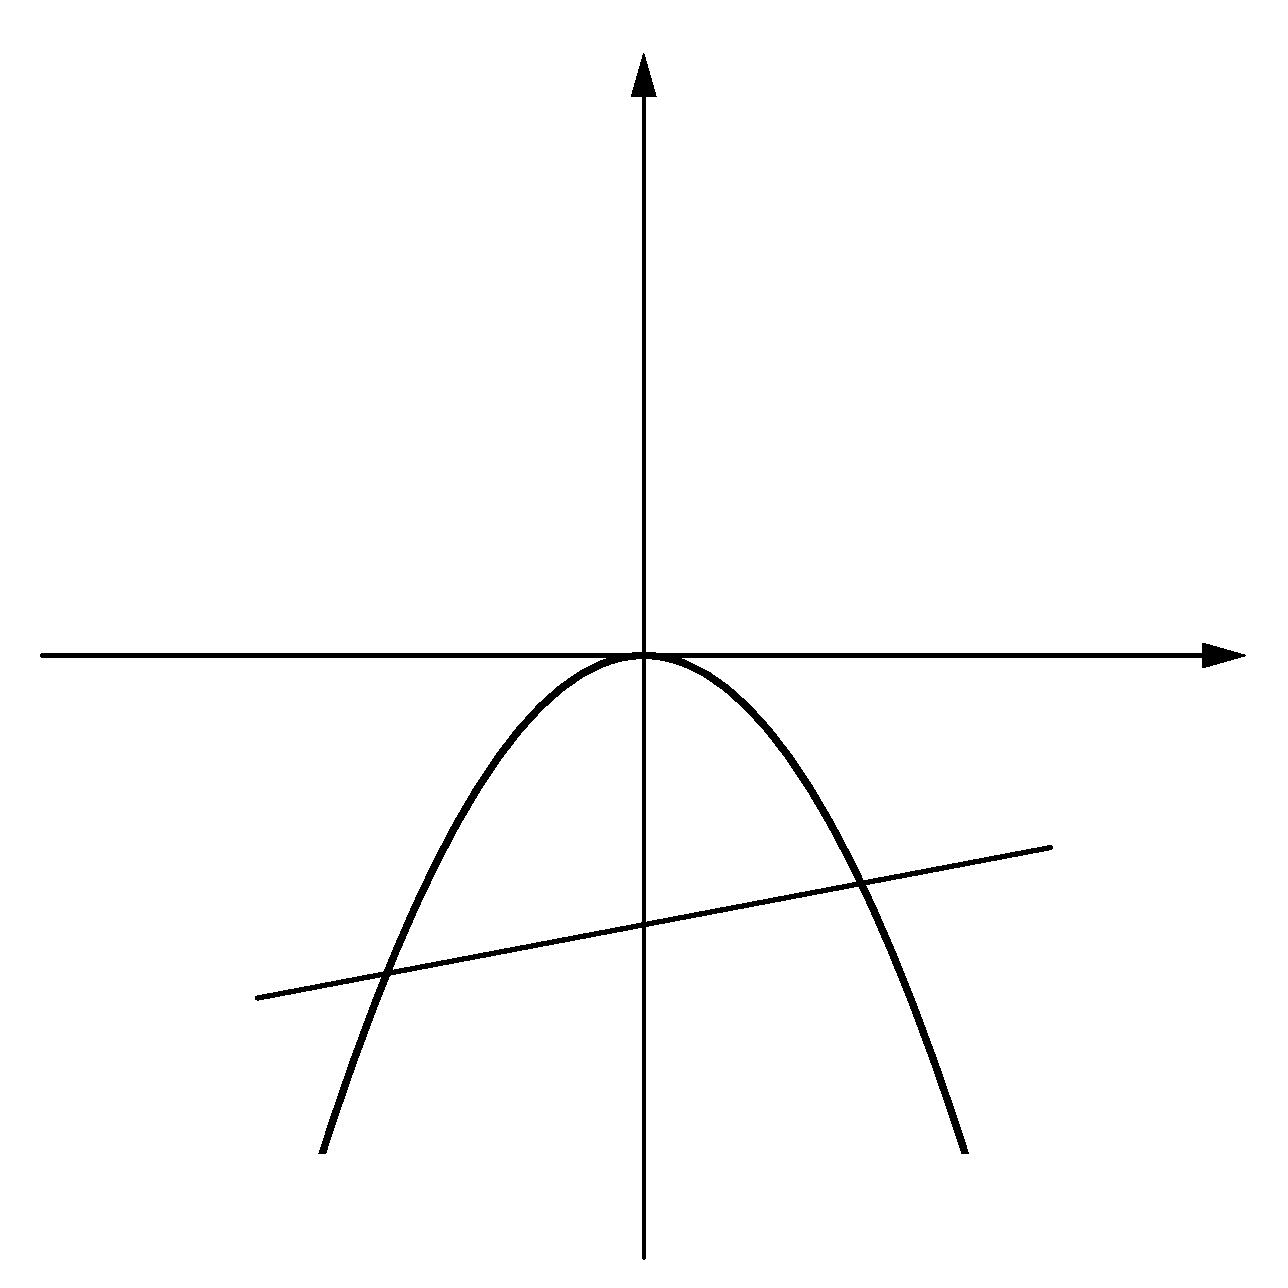
\includegraphics[scale=0.2]{5.28.pdf}
        \end{figure}
        \item \begin{align*}
            f(x)\text{是凹函数} & \iff f[\lambda x+(1-\lambda)y] \geq \lambda f(x)+(1-\lambda)f(y)\\
            &\iff -f[\lambda x+(1-\lambda)y] \leq -\lambda f(x)-(1-\lambda)f(y)\\
            & \iff g[\lambda x+(1-\lambda)y] \leq \lambda g(x)+(1-\lambda)g(y)\\
            &\iff g(x)\text{是凸函数}
        \end{align*}
    \end{enumerate}
    \item \sol
    \begin{enumerate}[label=\alph*)]
        \item $E(X_1) < E(X_2)$无法说明一定能获利,故无法说明存在套利.
        \item $P(X_2>X_1)>0$无法说明一定能获利,故无法说明存在套利.
    \end{enumerate}
\end{enumerate}
\clearpage